\documentclass[a4paper,12pt]{article}
\usepackage[indonesian]{babel}
\usepackage{graphicx}
\usepackage{multirow}
\usepackage{enumitem}
\usepackage{listings}
\usepackage{wrapfig}
\usepackage[T1]{fontenc}
\usepackage{inconsolata}
\usepackage{lipsum}
\usepackage{adjustbox}


\usepackage{color}
\usepackage[table]{xcolor}
\definecolor{mygreen}{rgb}{0,0.6,0}
\definecolor{mygray}{rgb}{0.5,0.5,0.5}
\definecolor{mymauve}{rgb}{0.58,0,0.82}
\lstset{%
    language=java,
    showstringspaces=false,          % Prevent tex replacing space to bracket in code
    frame=single,                    % Set frame around code
    backgroundcolor=\color{white},   % choose the background color
    basicstyle=\footnotesize,        % size of fonts used for the code
    breaklines=true,                 % automatic line breaking only at whitespace
    captionpos=b,                    % sets the caption-position to bottom
    commentstyle=\color{mygreen},    % comment style
    keywordstyle=\color{blue},       % keyword style
    stringstyle=\color{mymauve},     % string literal style
    numbers=left,
}

\graphicspath{ {./img/} }
\begin{document}
\title{ {\Large Laporan Praktikum}\\ Struktur Data\\{\Large Pertemuan 1}}

\author{Aldzikri Dwijayanto Prathama
    \\195410189
    \\Informatika}
\makeatletter
\begin{titlepage}
    \begin{center}
        {\huge \bfseries \@title}\\[14ex]
        
\includegraphics[scale=.8]{logo}\\[4ex]
        {\large \@author}\\[12ex]
        {\large \bfseries {SEKOLAH TINGGI MANAJEMEN INFORMATIKA DAN KOMPUTER
            AKAKOM YOGYAKARTA}}
    \end{center}


%{\large \@date}
\end{titlepage}
\makeatother
%\maketitle
\newpage
\tableofcontents
\newpage

\section{Tujuan}
Mahasiswa dapat menggunakan berbagai tipe data untuk menyimpan data baik aphabetic, 
aplhanumerik, maupun boolean
\section{Teori}
 
Setiap bahasa pemrograman memiliki tipe data yang spesifik. Tipe data akan 
digunakan untuk mendeklarasikan variable yang digunakan. Tipe data digunakan untuk 
menentukan bentuk data yag dapat ditampung oleh sebuah variabel.\\
 
Dalam java terdapat dua jenis tipe data. Yang pertama adalah tipe data primitive 
yang merupakan tipe data bawaan dari compiler java. Tipe data ini akan anda pelajari 
pada modul 1 ini.\\ 
 
Sedangkan tipe data yang kedua adalah tipe data buatan yang baru akan anda 
pelajari pada modul 2.\\
 
Dalam bahasa Java, tipe data primitive dibedakan menjadi tiga bagian yaitu:
\begin{enumerate}[label=\bfseries\arabic*.]
    \item \textbf{Tipe Data Alphabetic}
        \begin{itemize}
           \item Char
           \item String
        \end{itemize}

    \item \textbf{Tipe Data Alphanumeric}
        \begin{enumerate}[label=\alph*. ]
                \item Tipe data Bilangan Bulat 
                    \begin{itemize}
                        \item Byte 
                        \item Short 
                        \item Int 
                        \item Long
                    \end{itemize}

                \item Tipe data Bilangan Pecahan
                    \begin{itemize}
                       \item Float
                       \item Double
                    \end{itemize}
        \end{enumerate}

    \item \textbf{Tipe Data Boolean}
\end{enumerate}

\newpage

\section{Pembahasan}
\subsection{Praktik}
\subsubsection{Praktik 1}
\begin{lstlisting}
public class pembagian {
 public static void main(String[] args) {
  int banyaknyaApel = 5;
  int jumlahAnak = 2;
  int perolehan;
  perolehan = banyaknyaApel / jumlahAnak;
  System.out.println("Masing2 mendapat = " + perolehan);
 }
}
\end{lstlisting}

\textbf{Tipe Data Integer}
Program di atas menghitung operasi pembagian 5 dengan 2, yang seharusnya menghasilkan 2,5.
Tetapi pada saat dijalankan hanya menghasilkan 2
\begin{center}
    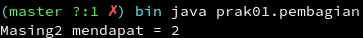
\includegraphics[scale=1]{1.png} 
\end{center}
Program tersebut hanya mengeluarkan angka 2, karena variabelnya menggunakan tipe
integer, yang hanya mampu menyimpan bilangan bulat.

\subsubsection{Praktik 2}
\begin{lstlisting}
public class cobaLong {
 public static void main(String[] args) {
  long coba = 1234567890123;
  System.out.println(coba);
 }
}
\end{lstlisting}

\textbf{Tipe Data Long}
Program diatas tidak bisa dieksekusi karena terjadi error
pada saat proses kompilasi.

\begin{center}
    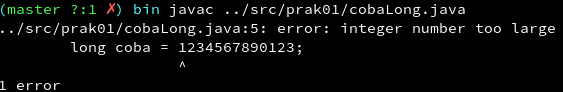
\includegraphics[width=\textwidth]{2.png}
\end{center}

Error tersebut terjadi karena compiler java mengira isi dari variabel coba
bertipe integer, sehingga nilai dari variabel tersebut harus ditambahkan L
untuk menyatakan bahwa nilai dari variabel bertipe long

\begin{lstlisting}
public class cobaLong {
 public static void main(String[] args) {
  long coba = 1234567890123;
  System.out.println(coba);
 }
}
\end{lstlisting}
Setelah nilai dari variabel ``coba'' ditambahkan dengan ``L'', program dapat
dikompilasi dan dijalankan

\begin{center}
    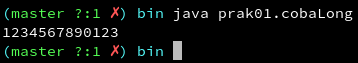
\includegraphics[scale=1]{3.png}
\end{center}

\subsubsection{Praktik 3}
\begin{lstlisting}
public class cobaKalimat {
 public static void main(String[] args) {
  char coba = "HAI";
  System.out.println(coba);
 }
} 
\end{lstlisting}

Program di atas tidak bisa dikompilasi, karena variabel coba bertipe char
yang hanya mampu menampung satu character, tetapi
diisi dengan 3 character.

\begin{center}
    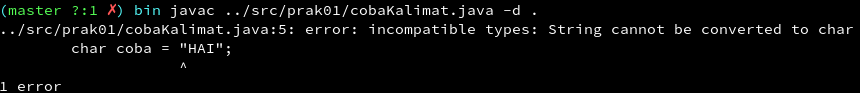
\includegraphics[width=\textwidth]{4.png}
\end{center}

Untuk variabel yang akan digunakan 
untuk menyimpan kalimat, gunakan tipe data String.
Sehingga kode yang benar adalah seperti berikut.

\begin{lstlisting}
public class cobaKalimat {
 public static void main(String[] args) {
  char coba = "HAI";
  System.out.println(coba);
 }
} 
\end{lstlisting}

Setelah dikoreksi kode bisa dicompile dan dijalankan

\begin{center}
    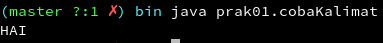
\includegraphics[width=\textwidth]{5.png} 
\end{center}
\newpage

\subsubsection{Praktik 4}
\begin{lstlisting}
public class Variabel {
 static int a;
 public static void main(String[] args) {
  int x;
  x = 10;
  a = 2;
  System.out.println("Nilai a : " + a);
  {
   int y;
   y = 5;
   System.out.println("Nilai x : " + x);
   System.out.println("Nilai a : " + a);
   {
    int z;
    z = 20;
    System.out.println("Nilai x + y + z + a :" + (x + y + z + a));
   }
   System.out.println("Nilai Z : " + Z);
   System.out.println("Nilai y : " + y);
  }
  System.out.println("Nilai Z : " + Z);
  System.out.println("Nilai y : " + y);
  System.out.println("Nilai x : " + x);
 }
}
\end{lstlisting}

\textbf{Lingkup Variabel}

Program tersebut tidak dapat dijalankan karena terjadi error
pada saat proses kompilasi.

\begin{center}
    
\includegraphics[width=\textwidth]{6.png}
\end{center}

Error tersebut terjadi karena java tidak bisa menemukan variabel z dan y.
pada baris 18 dan 21, terdapat perintah untuk menampilkan nilai dari variabel z,
tetapi perintah tersebut ditulis di luar curly braces di mana variabel z
dideklarasikan. Lalu pada baris 22 terdapat perintah untuk menampilkan nilai
dari variabel y, tetapi juga ditulis diluar curly brace dimana variabel y 
dideklarasikan. Karena perintah yang mengambil nilai dari variabel z dan y
ditulis di luar curly braces di mana kedua variabel tersebut dideklarasikan,
maka java tidak bisa menemukan kedua variabel tersebut.\\

Setelah baris perintah yang bermasalah dihapus, kode menjadi seperti berikut.
\begin{lstlisting}
public class Variabel2 {
 static int a;
 public static void main(String[] args) {
  int x;
  x = 10;
  a = 2;
  System.out.println("Nilai a : " + a);
  {
   int y;
   y = 5;
   System.out.println("Nilai x : " + x);
   System.out.println("Nilai a : " + a);
   {
    int z;
    z = 20;
    System.out.println("Nilai x + y + z + a :" + (x + y + z + a));
   }
   System.out.println("Nilai y : " + y);
  }
  System.out.println("Nilai x : " + x);
 }
}
\end{lstlisting}

Setelah kode dibetulkan, program dapat dijalankan.

\begin{center}
    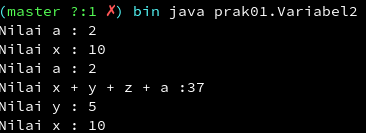
\includegraphics[width=\textwidth]{7.png} 
\end{center}

\subsubsection{Praktik 5}
\begin{lstlisting}
import java.util.Scanner;

public class inputDataViaKeyboard {
    public static void main(String[] args) {
        String nama;
        String alamat;
        int umur;
        char jekel; // jenis kelamin
        String hobi[] = new String[3];
        float ipk;
        Scanner masukan = new Scanner(System.in);
        int bacaTombol = 0;
        System.out.print("Silakan masukkan nama anda : ");
        nama = masukan.next();
        System.out.print("Silakan masukkan alamat anda : ");
        alamat = masukan.next();
        System.out.print("Silakan masukkan umur anda : ");
        umur = masukan.nextInt();
        System.out.print("Silakan masukkan Jenis Kelamin anda : ");
        try
        {
            bacaTombol = System.in.read();
        }
        catch (java.io.IOException e)
        {
        }
        jekel = (char) bacaTombol;
        System.out.println("Silakan masukkan hobi (maks 3) : ");
        System.out.print("hobi ke-0 : ");
        hobi[0] = masukan.next();
        System.out.print("hobi ke-1 : ");
        hobi[1] = masukan.next();
        System.out.print("hobi ke-2 : ");
        hobi[2] = masukan.next();
        System.out.print("Silakan masukkan IPK anda : ");
        ipk = masukan.nextFloat();
        System.out.println("Nama anda adalah " + nama);
        System.out.println("Nama alamat adalah " + alamat);
        System.out.println("Umur anda adalah " + umur);
        System.out.println("Jenis Kelamin anda adalah " + jekel);
        System.out.println("Hobi ke-0 anda adalah " + hobi[0]);
        System.out.println("Hobi ke-1 anda adalah " + hobi[1]);
        System.out.println("Hobi ke-2 anda adalah " + hobi[2]);
        System.out.println("IPK anda adalah " + ipk);
    }
}
\end{lstlisting}

Program diatas merupakan program yang menerima input dari user.
Yang membedakan program tersebut dengan praktik sebelumnya
antara lain try-catch-finally, dan System.in.read().\\

Perintah try-cath tersebut disebut exception.
try berisi perintah yang digunakan untuk mencoba
terjadinya error.
sedangkan catch berisi perintah yang dijalankan bila error terjadi.\\

Perintah System.in.read() berguna untuk membaca unicode dari character,
misalnya A unicodenya adalah 65, dan a unicodenya 97.\\

lalu untuk merubah unicode menjadi char dan menyimpannya ke variabel
bisa menggunakan\\
variabel\_Char = (char)variabel\_Unicode;\\

Jika program pada praktik 5 ini dijalankan, hasilnya seperti berikut.
\begin{center}
    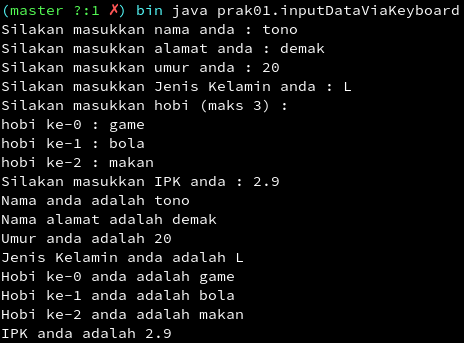
\includegraphics[width=\textwidth]{8.png} 
\end{center}

\subsection{Latihan}
\begin{lstlisting}
import java.util.Scanner;
public class Latihan {
   public static void main(String[] args) {
       Scanner in = new Scanner(System.in);
       System.out.printf("Masukkan password: ");
       String password = in.next();
       if(password.equalsIgnoreCase("akakom")){
           System.out.printf("Pasword anda benar \n");
       }else{
           System.out.printf("Pasword anda salah \n");
       }
   }
}
\end{lstlisting}

Program pada latihan merupakan program yang akan mengecek
apakah password yang dimasukkan oleh user berisi kalimat
akakom, atau bukan. Untuk mencocokan dua string dan
bersifat case-insensitive digunakan fungsi equalsIgnoreCase.

\begin{center}
    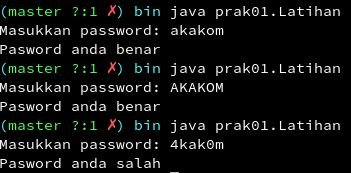
\includegraphics[width=\textwidth]{9.png} 
\end{center}

\subsection{Tugas}
Untuk tugas mahasiswa membuat program seperti pada praktik 5,
tetapi program diubah agar bisa menyimpan data diri minimal
5 orang mahasiswa.
\begin{lstlisting}
import java.io.IOException;
import java.util.Scanner;

public class Tugas {

    public static void main(String[] args) {
        Scanner in = new Scanner(System.in);
        System.out.print("Banyak mahasiswa = ");
        int mahasiswa = in.nextInt();
        String[] nama = new String[mahasiswa];
        String[] alamat = new String[mahasiswa];
        int[] umur = new int[mahasiswa];
        char[] jekel = new char[mahasiswa];
        String[][] hobi = new String[mahasiswa][3];
        float[] ipk = new float[mahasiswa];
        int bacaTombol = 0;
        for(int i=0; i<mahasiswa; i++){
            System.out.print("Masukkan nama: ");
            nama[i] = in.next();

            System.out.print("Masukkan alamat: ");
            alamat[i] = in.next();

            System.out.print("Masukkan umur: ");
            umur[i] = in.nextInt();

            System.out.print("Masukkan jenis kelamin: ");
            try{
                bacaTombol = System.in.read();
            }
            catch(IOException e){
            }
            jekel[i] = (char) bacaTombol;

            System.out.println("Masukkan hobi (maks 3)");
            for(int j=0; j<3; j++){
                System.out.print("Masukkan hobi ke-"+j+": ");
                hobi[i][j]=in.next();
            }

            System.out.print("Masukkan IPK: ");
            ipk[i] = in.nextFloat();

            System.out.printf("\n \n");
        }
        for(int i=0; i<mahasiswa; i++){
            System.out.println("Nama: "+nama[i]);
            System.out.println("Alamat: "+alamat[i]);
            System.out.println("Umur: "+umur[i]);
            System.out.println("Jenis kelamin"+jekel[i]);
            for(int j=0; j<3; j++){
                System.out.println("Hobi ke-"+j+": "+hobi[i][j]);
            }
            System.out.println("IPK: "+ipk[i]);
            System.out.printf("\n");
        }
    }
}
\end{lstlisting}

Program di atas hampir sama dengan program pada praktik 5, hanya saja variabel
diubah menjadi array, yang panjangnya sama dengan nilai di variabel mahasiswa.
Sedangkan untuk variabel hobby, karena setiap orang maksimal memasukkan 3 hobi
maka variabelnya diubah menjadi array 2 dimensi dengan jumlah baris sama dengan
jumlah mahasiswa dan jumlah kolom sebanyak 3.\\

Karena variabel diubah menjadi array, maka digunakan perulangan for untuk memasukkan
nilai ke variabel.\\

sehingga jika program dijalankan seperti berikut:\\
\begin{center}
    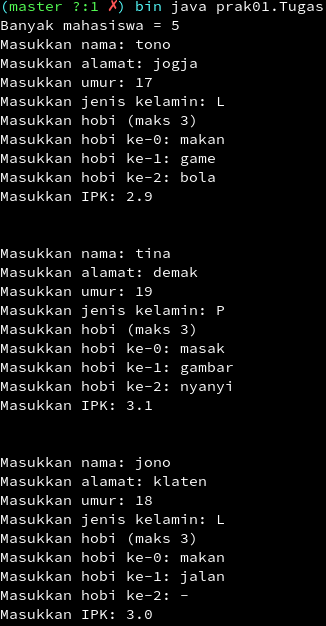
\includegraphics[scale=1]{tugas01.png} 
    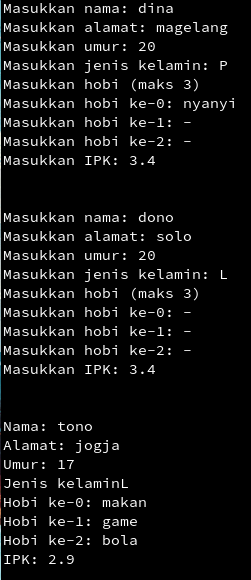
\includegraphics[scale=1]{tugas02.png} 
    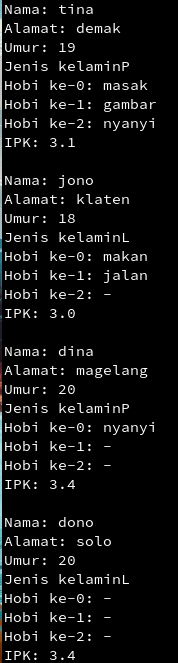
\includegraphics[scale=1]{tugas03.png} 
\end{center}

\newpage

\section{Kesimpulan}
Setelah praktik mahasiswa dapat menggunakan berbagai tipe data untuk menyimpan data baik alphabetic, alphanumeric,
maupun boolean.
\end{document}
